\chapter{System Design}
% Provide a detailed explanation of the overall system architecture
% \cite{lin1991divergence}, i.e. the HOW of the project.
% Use UML, system architecture diagrams, screenshots, code snippets 
% and algorithms to illustrate your design.

In this chapter, I will be discussing how when about designing my project
and the design principles I used throughout.
I will provide diagrams and screenshots of various components,
and show implementation snippets of code.

\begin{figure}[h!]
    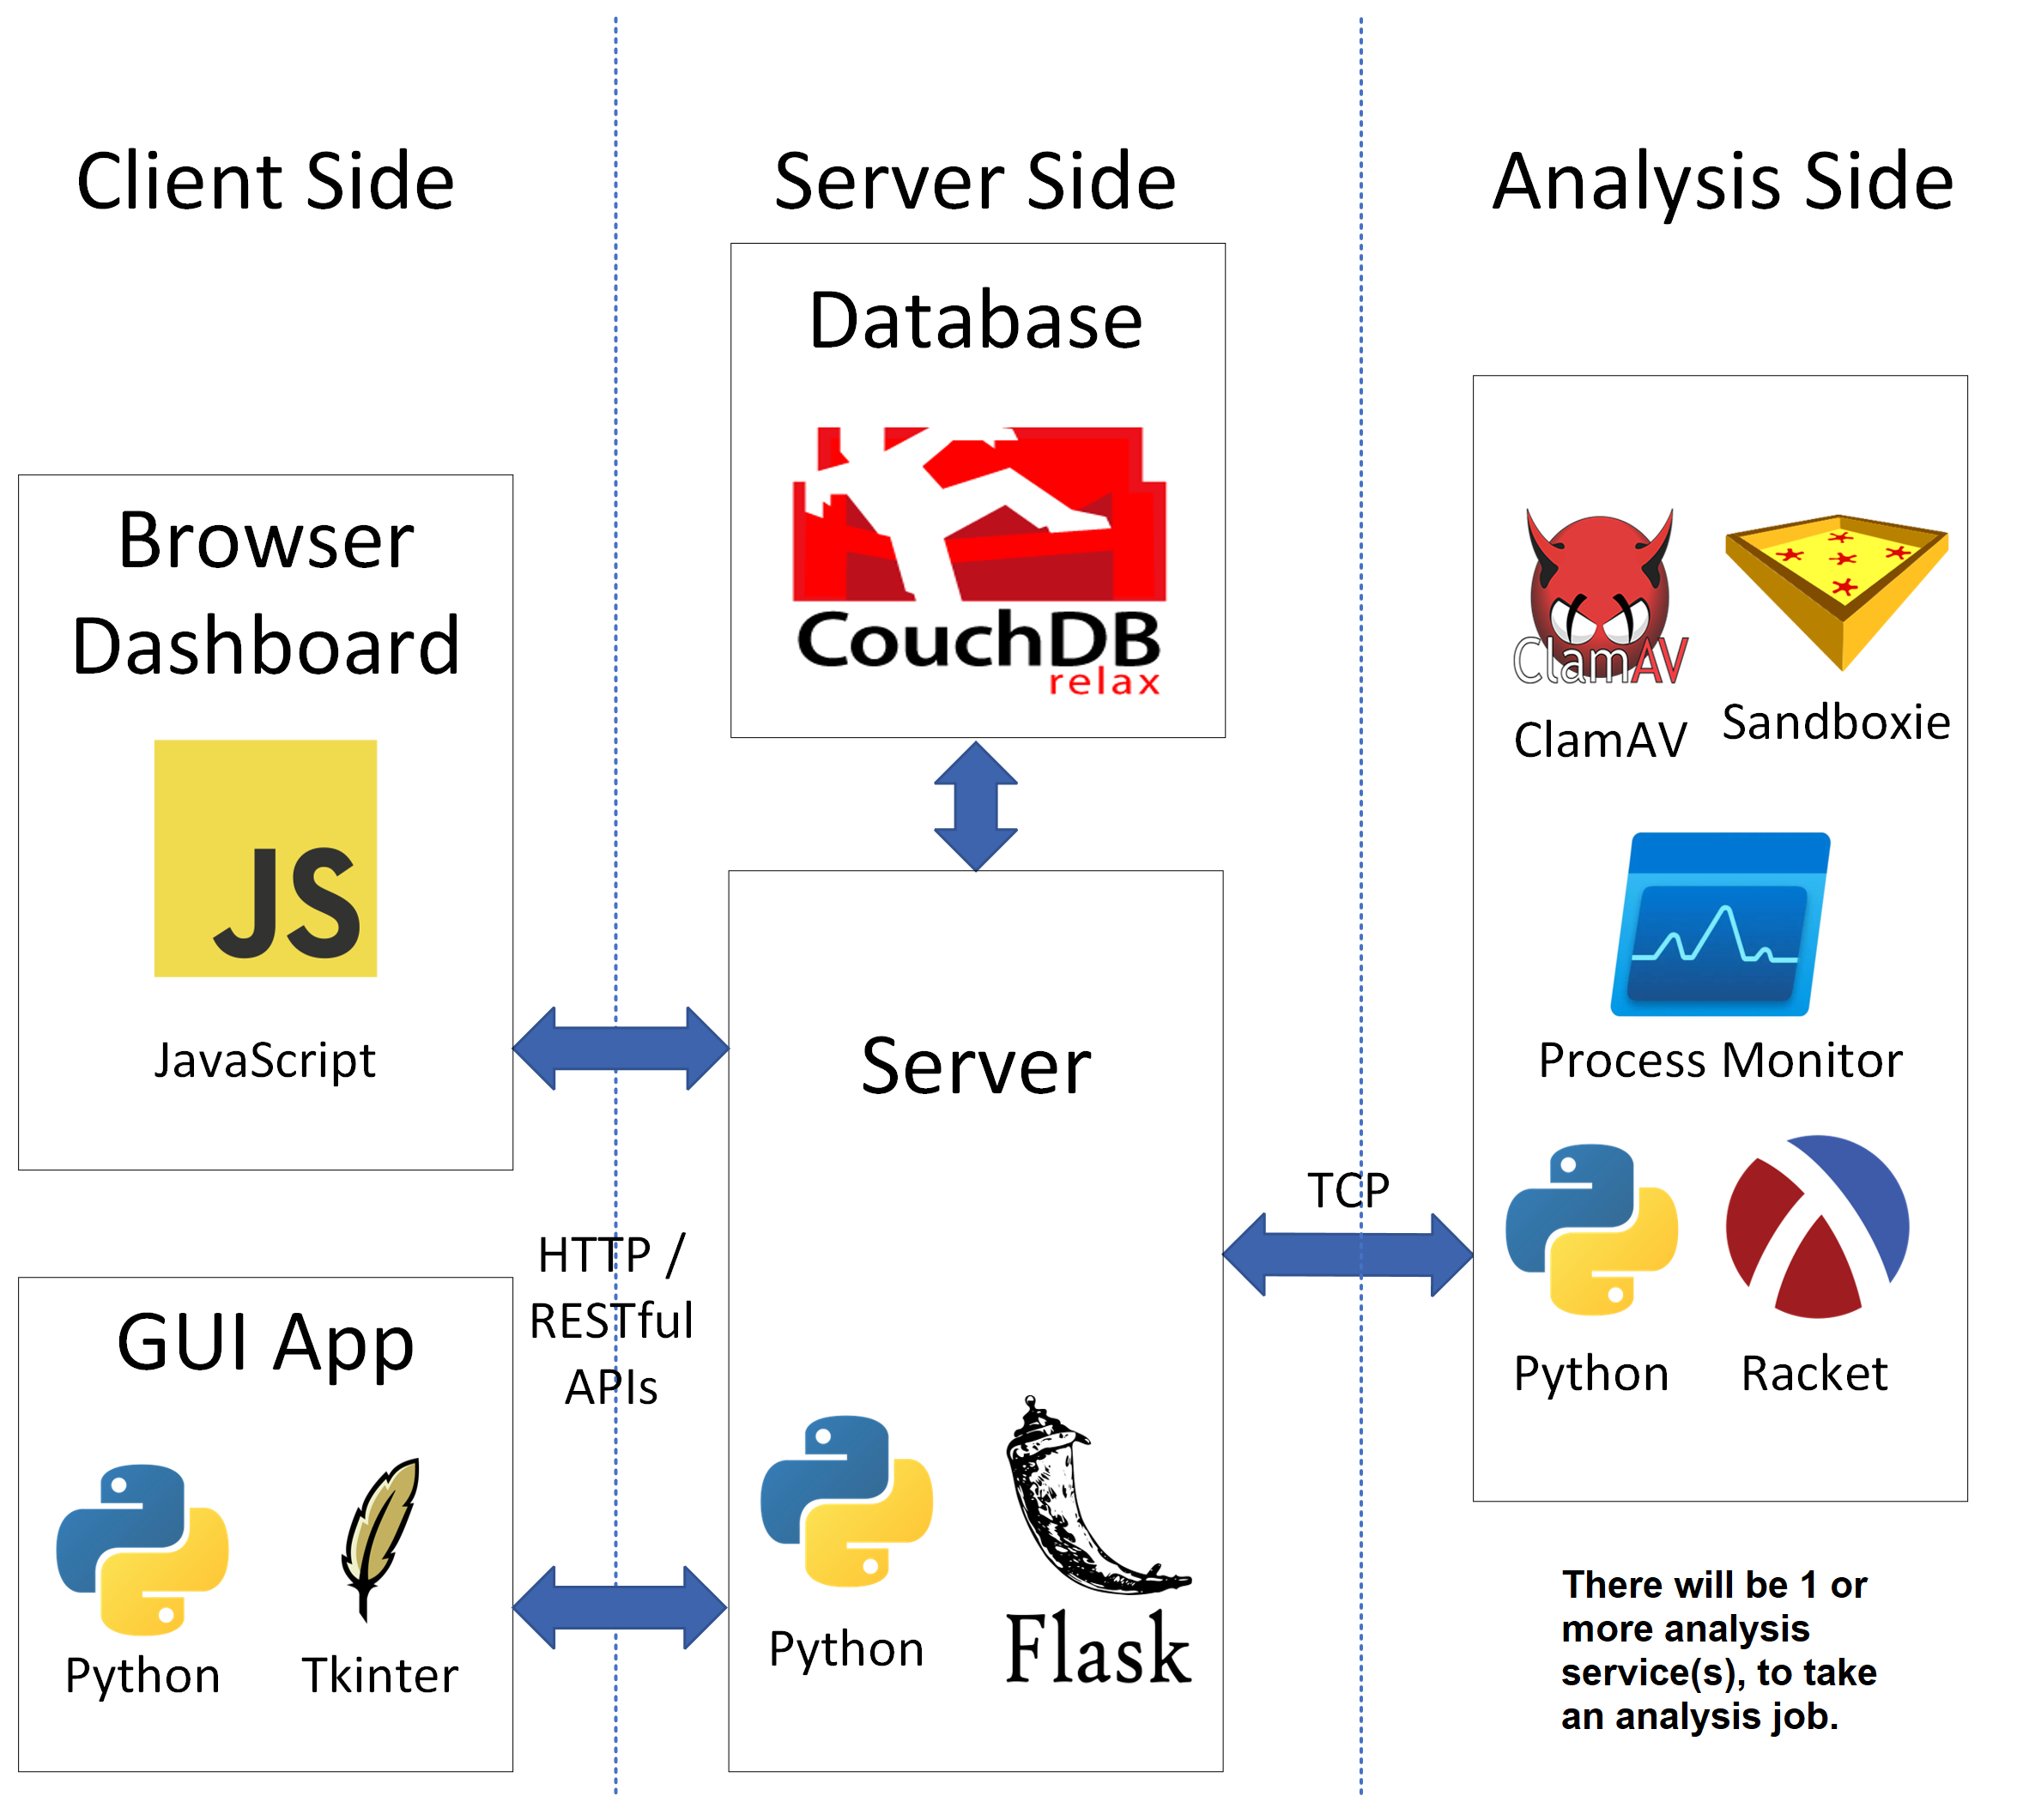
\includegraphics[width=0.9\textwidth]{images/diagrams/architecture}
    \caption{System Architecture Diagram}
    \label{image:sysArchitecture}
\end{figure}

Below you can see a system architecture diagram when in execution the platform can be broken down into three parts the client, server and sandbox side.

\section{Windows GUI Application}
Python files with the \texttt{frame.py} suffix contain Tkinter frame classes,
and each of these files contains only one class that inherits the Tkinter frame class.

\subsection{User Interface}
The client post-provisioning features a Tkinter \texttt{Notebook},
with 3 sub-frames, Main Page ("Caladium"), Quarantine and Preferences.
You can navigate through these by clicking on each label on the window.
The \texttt{Notebook} Tkinter widget allows you to
group frames together allowing navigation between them.

The Main Page in the frame features a button to manually scan a file,
and a label indicating the current scanning directory.


\subsubsection{Quarantine Page}

\begin{figure}[h!]
    \centering
    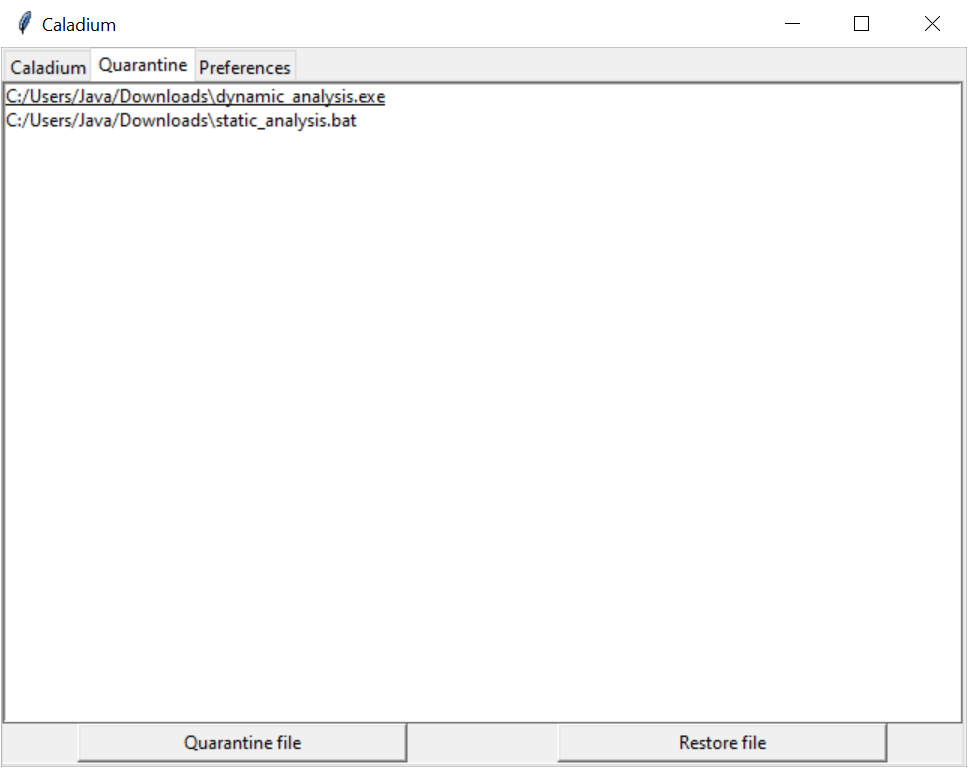
\includegraphics[width=0.75\textwidth]{../docs/client.png}
    \caption{Quarantine Page Screenshot}
    \label{image:quarantinePageScreenshot}
\end{figure}

\subsubsection{Preferences Page}

\subsubsection{Scanning Frame}

\subsection{Quarantine}
When files are added to the quarantine they are encrypted with an XOR cipher to avoid accidental execution of malware, in the event of the user accidentally stumbling upon the location of the quarantine.

\subsection{Directory Scanning}
The client has the ability to identify newly downloaded files,
this is implemented in \texttt{client/src/dirchangelistener.py}.
This functionality is achieved by scanning for new files in a directory.

The implementation contains a class called \texttt{DirChangeListener}
an instance of this class will be made and passed a callback function that
will be called when a new file appears in the directory.

A \textbf{tkthread} thread is spawned which loops
and checks for new files on every iteration.
The current directory state is obtained using
\texttt{os.listdir(dir\_name)} and compared to the last state.
To prevent the application from locking up,
the Tkinter GUI is given some time to render on each iteration.
This will be explained in more detail below.

\subsection{Thread Model}

\section{Server Dashboard}
The dashboard is a single-page web application (SPA) it is fully written in JavaScript.
This means when you navigate to another page in the dashboard it doesn't have to pull it from the server, just fetch the data specific to that page, then render it dynamically using JavaScript.

\begin{figure}[h!]
    \centering
    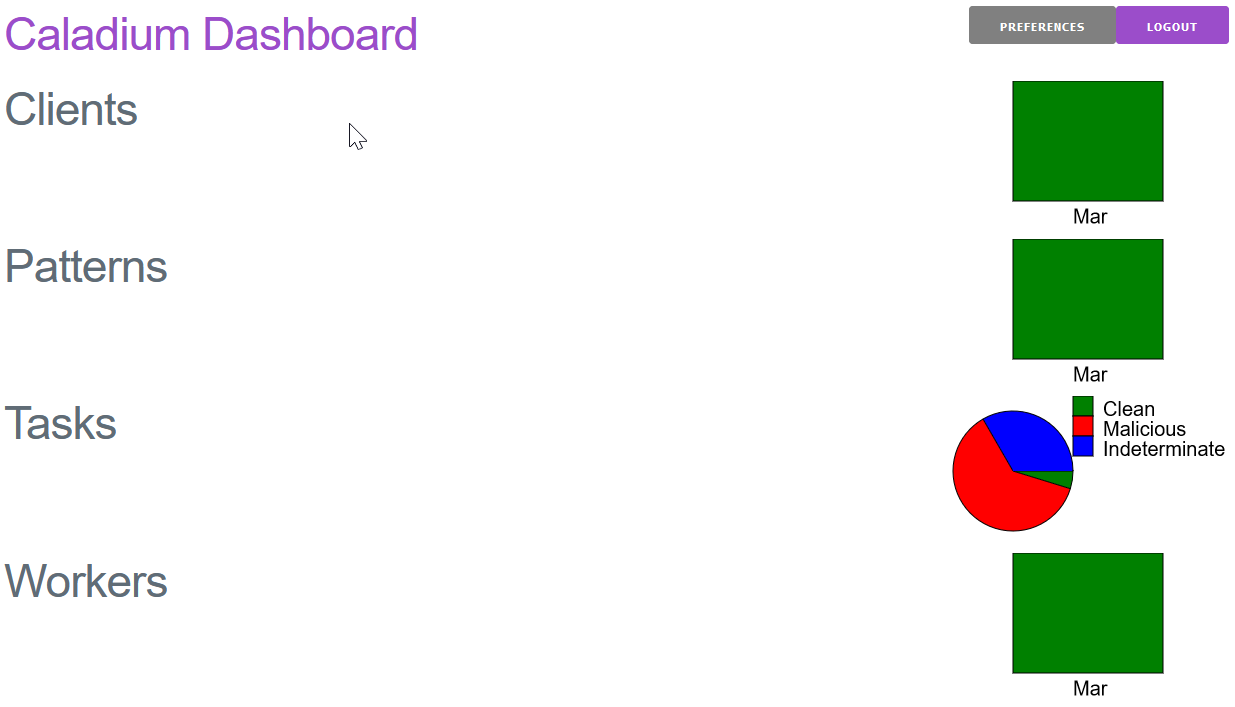
\includegraphics[width=0.75\textwidth]{../docs/dashboard.png}
    \caption{Dashboard Index Screenshot}
    \label{image:dashboardScreenshot}
\end{figure}

Upon loading a new page, the contents of the page are
dynamically generated using DOM Lisp expressions.
The URL of the page is then updated using the History API.

In the \textbf{server/static/js/index.js} I have a dictionary called
\textbf{routes} containing a list of all the routes and their corresponding
page classes and their URL.
When the page is loaded, the URL is checked against the dictionary
and the corresponding page class is loaded.

And doesn't make use of any external libraries.
I made this decision early because I wanted to keep the project as self-contained as possible.

\subsection {Page Class Hierarchy}

\begin{figure}[h!]
    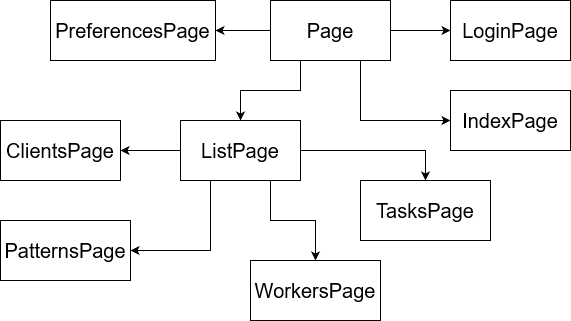
\includegraphics[width=0.9\textwidth]{images/diagrams/dashboard_hierarchy.drawio}
    \caption{Page Class Hierarchy Diagram}
    \label{image:sysArchitecture}
\end{figure}

The dashboard is object-oriented,
all of the main code can be found in the \textbf{server/static/js/index.js} file.
This contains code for communicating with the server endpoints and classes for each page.

All pages inherit the \textbf{Page} class,
as they share common functionality which upholds the DRY principle.

Each page class must implement the \textbf{loadPage} method,
which is called when the page is loaded.
This can be used for fetching data from the backend.

\subsection{DOM Lisp Expressions}
In a single-page application (SPA), all page content is dynamically generated without
need to pull HTML from a server when navigating between pages.

Initially, I considered embedding raw HTML within JavaScript code,
but found it to be inelegant.
As a solution, I created a domain-specific language (DSL)
to represent the Document Object Model (DOM) as Lisp expressions.

My approach involved storing these Lisp expressions as strings within each page class,
and including parameters which could be replaced with their actual values during page loading.
This approach allowed me to encapsulate DOM expressions within each page class.

This DSL approach simplifies the creation and maintenance of code by providing a higher level of abstraction,
making the syntax for creating DOM elements more readable and understandable.

I developed a library, that can be found at \textbf{server/src/static/js/pantothenic.js},
which includes the \textbf{generateDOM} function that takes a
DOM Lisp expression and parameters,
and returns a DOM object.

The DOM is a tree of nested components that represents web applications within a browser.
By using Lisp expressions as a DSL to represent DOMs,
I have created a more elegant solution to generating dynamic
content within a single-page application.

Below you will find an example of a DOM Lisp expression.
This is taken from the \textbf{Preferences} class in the
\textbf{server/src/static/js/index.js} file.
It is a list of components for the HTML page,
including an input box for a new password for the admin user
and a button that toggles the auto-provisioning of new users.
When the user clicks the button, it calls the
\textbf{toggleAutoProvision} method within the class.

\begin{lstlisting}
this.body = ` (div (hash "children"
                (list
                    navigationBar
                    (input (hash "type" "password" "id"
                        "newPassword" "placeholder" "New Password"))
                    (button (hash "onclick" changePasswordOnClick
                        "innerHTML" "Update Password"))
                    (hr)
                    (button (hash "onclick" toggleAutoProvision
                        "innerHTML" autoProvisionButtonText)))))`;
\end{lstlisting}

\section{Server Side}

\subsection{Server Endpoints}
The server uses the Flask micro-framework to provide the RESTful API.
I decided to categorise the API into five sections:
clients, databases, patterns, tasks and workers.
Flask supports a feature called blueprints,
which allows you to split your web application into multiple components.
I used a blueprint for each of the five sections of the API,
and each blueprint is stored in a separate file.

This is an example of a blueprint taken from the worker's blueprint.
\begin{lstlisting}[language=python]
...

import flask

...

workers = flask.Blueprint(__name__, "workers")

@workers.get("/api/workers")
def get_records_route():
    return database.get_caladium_collection("workers")

...
\end{lstlisting}

Each of the endpoints is RESTful the HTTP method name signifies the type operation to be performed on that resource, the table below will show each method and a description of each.

Each

\begin{table}
    \centering
    \begin{tabular}{|p{2cm}|p{6cm}|}
        \hline
        \multicolumn{2}{|c|}{HTTP Methods and Descriptions} \\
        \hline
        Method & Description\\
        \hline
        GET & Fetches data from a server\\
        \hline
        POST & Creates new data on the server\\
        \hline
        PUT & Update existing data on the server\\
        \hline
        DELETE & Delete a record by ID\\
        \hline
    \end{tabular}
    \caption{HTTP Methods and Descriptions}
    \label{table:httpmethods}
\end{table}

\subsection{Authentication}

\section{Analysis Side}
The main file of the analysis side can be found in \texttt{sandbox/src/main.rkt},
it is written in the Racket language, when it begins it will open a TCP port ready to accept incoming requests

\subsection{Communication with Server Side}
When a client asks the server to analyze a file,
the server needs to assign the job to one of its worker instances.
To keep track of what the workers are doing,
the server needs a way to communicate with them in real time.
I chose to use TCP for this purpose,
a communication method that allows data to be sent and received between devices.

The main program for analyzing the file is written in Racket,
which has built-in support for TCP. The server is written entirely in Python,
which also supports TCP using the sockets library.
However, I encountered a problem when trying to receive information from the workers.
The server had no way of knowing how much data was being sent,
so I looked for a solution and found a
helpful answer on Stack Overflow \cite{chqrlie:2022}
The solution was to include the length of the incoming
data at the beginning of the packet
so that the server would know how much data to expect.

\section{Scanning Process}
When a file is passed to the analysis worker from the server,
the scanning process begins as seen in diagram \ref{image:scanningProcess}.
Malicious patterns are also passed to the worker.

\begin{figure}[h!]
    \centering
    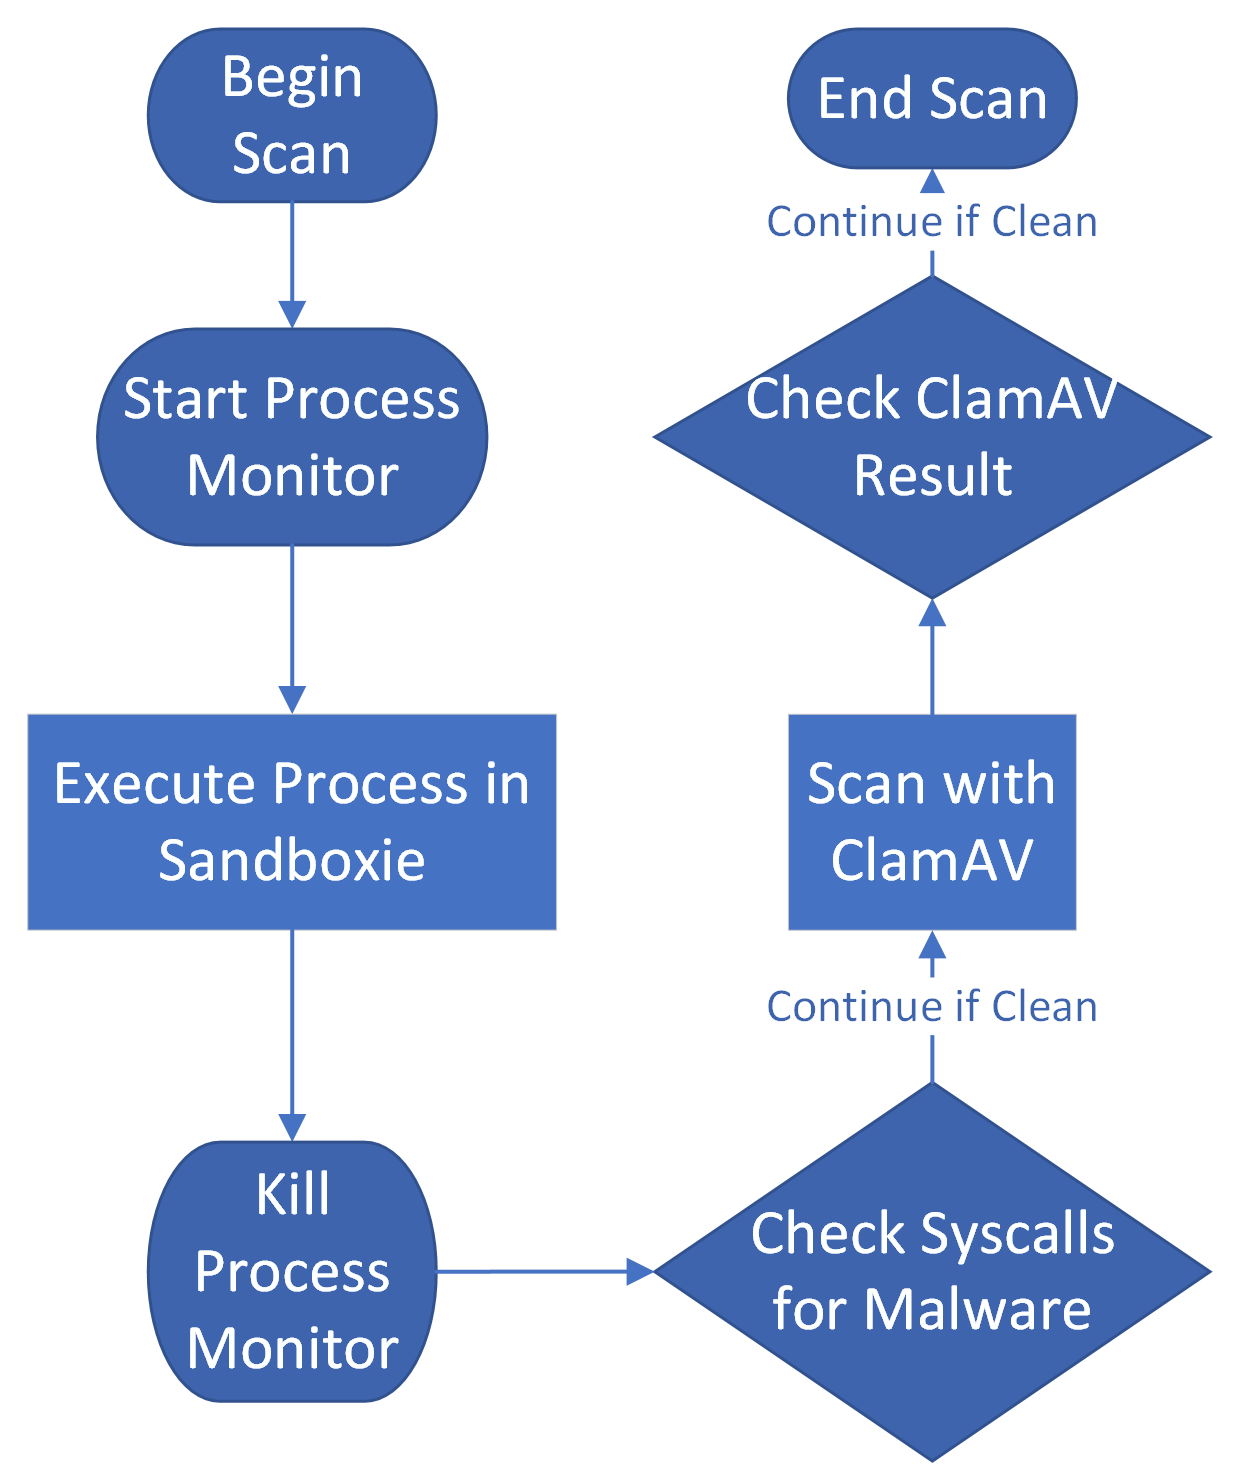
\includegraphics[width=0.5\textwidth]{images/diagrams/scan_process}
    \caption{Scanning Process Diagram}
    \label{image:scanningProcess}
\end{figure}

The first part of the process is dynamic analysis.
It begins by spawning a Process Monitor,
then the target file is executed in Sandboxie.
While this is happening,
Process Monitor is logging the system calls performed by the target file.
Once the process is finished or a certain amount of time elapses (timeout),
the process monitor is killed. This will return a list of system calls in CSV format.

We must iterate through all these system calls to see if we
get a match with one of the patterns that were passed to the worker.
If there isn't a match, we will continue to the next stage of the process,
the static analysis.

This is done with ClamAV, which will be passed to the
\texttt{clamscan.exe} as a parameter.
We will check the output of this to see if it's malicious. If none detect anything,
the scan will end and the file can be deemed clean.
Each state of the process gives updates back to the server along with
text messages that will be presented to the client.
